\chapter{Specialising and optimising xDSL pattern rewriting}
\label{chap:specialising-optimising-pattern-rewriting}

%% What is the goal
% Hook
In \autoref{chap:measuring-compiler-performance}, we constructed a set of experiments to empirically compare the performance of the xDSL and MLIR compiler frameworks.
% Argument
The goal of these experiments is to use xDSL and MLIR as proxies to characterise the performance of static and dynamic languages for the implementation of user-extensible compiler frameworks.
However, these experiments do not exactly capture this goal. We argue this is because they are measuring both the implementation details of the framework in addition to the runtime of the language, with the former obscuring our goal of measuring the latter. In this chapter, we mitigate this by specialising the xDSL framework to implement only a single workload. This elides aspects of the implementation which provide expressivity at the cost of performance, and is representative of the best-case performance of Python for this workload.
% Link
The benefits of this specialisation are twofold. Firstly it reveals inefficiencies in xDSL which can be optimised to improve the general performance of the framework. Secondly, it provides a true performance baseline for dynamic languages irrespective of implementation details which can be used to quantify the impact of dynamism in \autoref{chap:dynamism-pattern-rewriting}.

\section{Micro-benchmarks}
\label{sec:specialising-ubenchmarks}

% Hook
In \autoref{chap:measuring-compiler-performance}, we developed a set of micro-benchmarks for xDSL to compare its performance on fundamental operations with MLIR.
% Argument
The small size of these micro-benchmarked fundamental operations makes them tractable first targets for manual specialisation and optimisation. Following this, the performance uplift as a result of these changes can be trivially characterised by repeating measurement of the micro-benchmark.
% Link
In this section, we examine the specialisation process for these micro-benchmarks in detail. % TODO: Add more stuff here!!

\subsection{Operation trait checks}
\label{ssec:specialising-ubenchmarks-trait}

% Hook
Chapter \ref{chap:measuring-compiler-performance} measured a slow-down of approximately $130\times$ from MLIR to xDSL for trait checking micro-benchmarks (\autoref{tab:ubenchmark-trait-checks}).
% Argument
% % Link
% There are two factors which contribute to this slow-down. The first is the inherent overhead incurred by the interpreter loop and data structures in Python's dynamic language runtime. The second is differences in implementation between xDSL and MLIR.
% Examining this micro-benchmark in detail allows us to decouple the performance contributions of the implementation and language runtime.
% % , and provides insight into the impact of dynamism on user-extensible compiler framework workloads.

\begin{figure}[H]
    \begin{subfigure}[b]{0.45\textwidth}
       \centering
        \begin{minted}[fontsize=\footnotesize]{python}
            @classmethod
            def has_trait(
                cls,
                trait: type[OpTrait] | OpTrait,
                *,
                value_if_unregistered: bool = True,
            ) -> bool:
                from xdsl.dialects.builtin import UnregisteredOp

                if issubclass(cls, UnregisteredOp):
                    return value_if_unregistered

                return cls.get_trait(trait) is not None
        \end{minted}
        \footnotesize\vspace{1.5em}
        \caption{Outer \mintinline{python}{has_trait} method.}
        \label{listing:ubenchmark-trait-checks-xdsl-has}
    \end{subfigure}
    \hfill
    \begin{subfigure}[b]{0.45\textwidth}
        \centering
        \begin{minted}[breakanywhere,fontsize=\footnotesize]{python}
            @classmethod
            def get_trait(
                cls,
                trait: type[OpTraitInvT] | OpTraitInvT
            ) -> OpTraitInvT | None:
                if isinstance(trait, type):
                    for t in cls.traits:
                        if isinstance(t, cast(
                            type[OpTraitInvT], trait
                        )):
                            return t
                else:
                    for t in cls.traits:
                        if t == trait:
                            return cast(OpTraitInvT, t)
                return None
        \end{minted}
        \caption{Inner \mintinline{python}{get_trait} method.}
        \label{listing:ubenchmark-trait-checks-xdsl-get}
    \end{subfigure}
    \vspace{1em}
    \captionsetup{name=Listing}
    \caption{xDSL methods implementing trait check functionality.}
    \label{listing:ubenchmark-trait-checks-xdsl}
\end{figure}

% Hook
In order to distinguish between the slow-down incurred by the language runtime as opposed to each approach's implementation, we leverage tracing profilers to examine the call stacks of the micro-benchmarks.
% Argument
In the xDSL implementation of \mintinline{python}{has_trait} (Listing \ref{listing:ubenchmark-trait-checks-xdsl}), we can see that approximately half of the operation is spent checking if the operation subclasses \mintinline{python}{UnregisteredOp} (\autoref{fig:ubenchmark-hastrait-xdsl-viztracer}).
Furthermore, \mintinline{python}{has_trait}s sub-invocation \mintinline{python}{get_trait} further incurs overhead with \mintinline{python}{isinstance} checks, \mintinline{python}{cast}ing and constructing iterators (\autoref{fig:ubenchmark-gettrait-xdsl-viztracer}).
% Link
This demonstrates that a significant proportion of the slow-down in xDSL's \mintinline{python}{has_trait} method is as a result of implementation details, as opposed to inherent limitations of Python's runtime.

\begin{figure}[H]
    \centering
    \begin{subfigure}[b]{\textwidth}
        \centering
        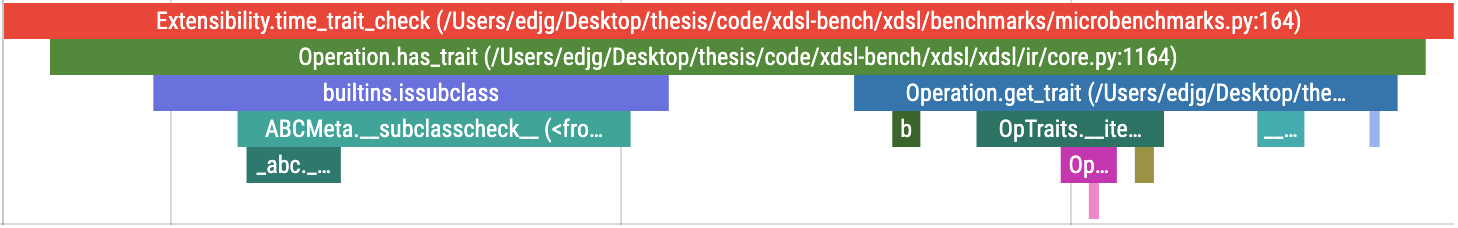
\includegraphics[width=\textwidth]{images/specialising_optimising_xdsl_rewriting/hastrait_xdsl_viztracer.png}
        \caption{Checking for \mintinline{python}{UnregisteredOp}s constitutes around half of \mintinline{python}{has_trait}s runtime.}
        \label{fig:ubenchmark-hastrait-xdsl-viztracer}
    \end{subfigure}
    \begin{subfigure}[b]{\textwidth}
        \centering
        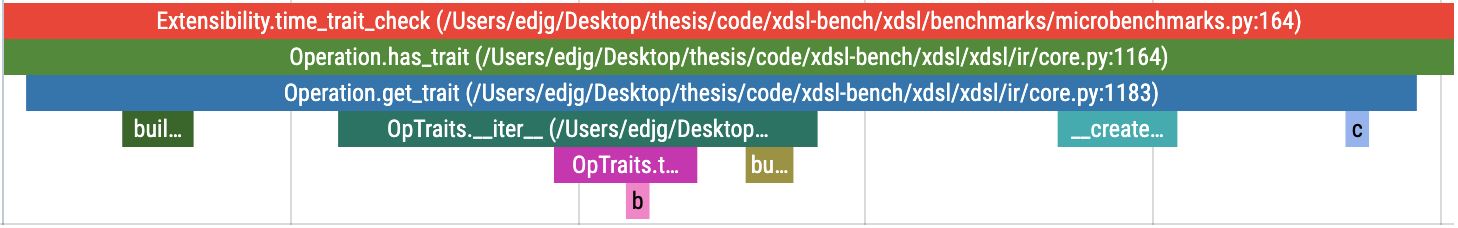
\includegraphics[width=\textwidth]{images/specialising_optimising_xdsl_rewriting/gettrait_xdsl_viztracer.png}
        \caption{\mintinline{python}{isinstance} checks, \mintinline{python}{cast}ing and constructing iterators constitutes around half of \mintinline{python}{get_trait}s runtime.}
        \label{fig:ubenchmark-gettrait-xdsl-viztracer}
    \end{subfigure}
    \caption{\texttt{viztracer} trace of xDSL's \mintinline{python}{has_trait} and \mintinline{python}{get_trait} methods.}
    \label{fig:ubenchmark-hasgettrait-xdsl-viztracer}
\end{figure}


%% TODO(Listing): Python bytecode vs perf disassembly?


% Hook
In order to measure the performance of only the language runtime
% Argument
By modifying xDSL's implementation to elide the extraneous code identified in the above traces (Listing \ref{listing:ubenchmark-trait-checks-both-xdsl}), we can improve its performance by a factor of eight (\autoref{tab:ubenchmark-trait-checks-optimised}).
This gives a number of insights into writing performant Python code in cases where it is unsuitable to dispatch to a lower level languages.
Firstly, even atomic operations such as function invocation and selection statements are slow in comparison to the runtime of the C++ implementation, coming as a result of the complexity of the evaluation loop of the CPython interpreter. % TODO: Consider \cite{}?
% This is substantiated by the bytecode profiles of the implementations (Appendix \ref{listing:bytecode-profiles-hastrait-original}, \ref{listing:bytecode-profiles-hastrait-optimised}), where each opcode represents in iteration of the evaluation loop.
In the case of \mintinline{python}{has_trait}, we address this by manually applying function inlining, and narrowing the trait argument from supporting both types and instances to only supporting types, eliminating selection of implementation between the two arguments. This minimises the number of opcodes and hence the number of cycles of the evaluation loop, improving performance.
% Link
Unfortunately, these approaches are in tension with writing expressive and terse code -- which are motivating factors for using Python.



\begin{table}[H]
  \caption{Trait checks in xDSL are approximately $130\times$ slower than in MLIR in the asymptotic case, but can be accelerated to $16\times$ slower with only algorithmic changes.} %, repeated ten times over $32768$ operations. Methodology is discussed in detail in Appendix \ref{} to facilitate replicability.}
  \label{tab:ubenchmark-trait-checks-optimised}
  \centering
  \begin{tabular}{ccc}
    \toprule
    \textbf{MLIR [ns]} & \textbf{xDSL [ns]} & \textbf{Optimised xDSL [ns]} \\
    \midrule
    $3.89 \pm 0.01$ & $504 \pm 76$ & $63.6 \pm 40$\\
    \bottomrule
  \end{tabular}
\end{table}



\begin{figure}[H]
    \centering
    \begin{subfigure}[b]{0.45\textwidth}
       \centering
        \begin{minted}[fontsize=\footnotesize]{python}
            has_trait = False
            for t in OP.traits._traits:
                if isinstance(t, TRAIT):
                    has_trait = True
                    break
        \end{minted}
        \footnotesize\vspace{5.5em}
        \captionsetup{name=Listing}
        \caption{xDSL's modified \mintinline{python}{has_trait} method.}
        \label{listing:ubenchmark-trait-checks-both-xdsl}
    \end{subfigure}
    \hfill
    \begin{subfigure}[b]{0.45\textwidth}
        \centering
        \begin{minted}[breakanywhere,fontsize=\footnotesize]{c++}
            template <template <typename T> class... Traits>
            inline bool hasTrait(TypeID traitID) {
                TypeID traitIDs[] = {TypeID::get<Traits>()...};
                for (unsigned i = 0, e = sizeof...(Traits); i != e; ++i)
                    if (traitIDs[i] == traitID)
                        return true;
                return false;
            }
            template <>
            inline bool hasTrait<>(TypeID traitID) {
                return false;
            }
        \end{minted}
        \captionsetup{name=Listing}
        \caption{MLIR's \mintinline{c++}{has_trait} method.}
        \label{listing:ubenchmark-trait-checks-both-mlir}
    \end{subfigure}
    \vspace{1em}
    \captionsetup{name=Listing}
    \caption{xDSL and MLIR methods searching trait arrays.}
    \label{listing:ubenchmark-trait-checks-both}
\end{figure}


\subsection{Operation instantiation}
\label{sec:specialising-ubenchmarks-instantiation}






%% Doesn;t add anything extra!!!
% \subsection{Operation traversal}
% \label{sec:specialising-ubenchmarks-traversal}




\section{Constant folding workload}

%%
% Hook
Having demonstrated specialisation as a technique to examine the underlying language runtime performance for micro-benchmarks, we can further apply it to real-world workloads such as constant folding.
% Argument
In this section, we specialise a simple pattern rewriter, constant folding over integer add operations (Listing \ref{listing:specialised-constant-kernel}). Unlike previous micro-benchmarks, MLIR's implementation of pattern rewriting also introduces non-negligible implementation overhead. As such, we provide a matching implementation of this algorithm in MLIR to guarantee fair comparison.
% Link
These specialised implementations can then be taken as performance baselines for their respective languages, and further analysed through bytecode tracing or disassembly to understand their implementation.

\vspace{2em}

\begin{code}
    \begin{minted}{python}
@dataclass
class ConstantFoldingIntegerAdditionPattern(RewritePattern):
    """Rewrite pattern that constant folds addition of integer types."""

    def match_and_rewrite(self, op: Operation, rewriter: PatternRewriter, /):
        # Only rewrite integer add operations
        if not isinstance(op, AddiOp):
            return

        # Ensure both operands are constants
        lhs_op: ConstantOp = op.operands[0].op
        rhs_op: ConstantOp = op.operands[1].op
        assert lhs_op.has_trait(ConstantLike)
        assert rhs_op.has_trait(ConstantLike)

        # Calculate the result of the addition
        lhs: int = lhs_op.value.value.data
        rhs: int = rhs_op.value.value.data
        folded_op = ConstantOp(
            IntegerAttr(lhs + rhs, op.result.type)
        )

        # Rewrite with the calculated result
        rewriter.replace_matched_op(folded_op, [folded_op.results[0]])
    \end{minted}
    \caption{xDSL implementation of a simple constant folding kernel.}
    \label{listing:specialised-constant-kernel}
\end{code}


\subsection{Specialisation}

%% Appendix for both xDSL and MLIR code?

%% Figure comparing traces
%%% One trace from unspecialised xDSL
%%% One trace from specialised xDSL


%% Table showing relative performance xDSL specialised / unspecialised vs MLIR

\begin{table}[H]
  \caption{.}
  \label{tab:ubenchmark-trait-checks-optimised}
  \centering
  \begin{tabular}{ccc}
    \toprule
    \textbf{MLIR [ns]} & \textbf{Unspecialised xDSL [ns]} & \textbf{Specialised xDSL [ns]} \\
    \midrule
    $3.89 \pm 0.01$ & $504 \pm 76$ & $63.6 \pm 40$\\
    \bottomrule
  \end{tabular}
\end{table}



%% Figure showing performance scaling


\subsection{Optimisation}

%% Introduction + scope of stuff
% Hook
% Argument
% xDSL is very big -- cannot optimise everything! But can show optimisations from specialisation are applicable and make change with time.
% Link

%% Removing overhead in functions
% Link
During the specialisation process \autoref{ssec:specialising-ubenchmarks-trait}, we saw that the implementation of xDSL's \texttt{has\_trait} helper function introduces significant overhead by checking the infrequent case of unregistered operations on the hot path of execution.
% Argument
Since this functionality was not used by the target workload, this could be elided by specialisation for performance. However, it also reveals an optimisation which can be applied to the general case:
% Link
% This optimisation was applied in \href{PR xyz}{PR xyz}, resulting in a $x\times$ speedup on micro-benchmarks and $y\times$ speedup on workload z.

%% Removing implicit builders

%% `__slots__` (stretch dataclasses stuff -> custom dataclass like thing without most of the overhead as a helper, replaces frozen dataclasses (what functionality is used here: https://github.com/python/cpython/blob/main/Lib/dataclasses.py and what can we rip out???))
